% !TeX root = ../../main.tex
% ------------------------------------------------------------------
%  4.2.2 Emplazamiento de cada componente.
%
%  Usa el mismo catálogo de la arquitectura lógica: 36 componentes, de
%  los cuales 13 van en nube, 11 en las instalaciones y 12 son híbridos
%  (ADR-03). La justificación de cada componente va en viñetas, la tabla
%  resume por dominio y criterio, y el detalle por elemento queda en el T-11.
% ------------------------------------------------------------------

\section{Emplazamiento de cada componente}
\phantomsection\label{fuente-02-a-emplazamiento}
\label{sec:emplazamiento}

El emplazamiento de cada componente se decide con los seis criterios del Artículo 16.2 de las Bases Administrativas (art. 16.2, p. 11): latencia tolerada, criticidad operacional, volumen de datos, restricciones regulatorias, disponibilidad de conectividad y costo total de propiedad. En este caso la conectividad y la latencia pesan más que en una operación de oficina, porque el caso describe una red que se corta: la fibra de Talca tiene en promedio cuatro cortes al año de hasta seis horas, Concepción carece de respaldo en la situación de partida, los cross-docking dependen de red móvil en la situación de partida y en Los Ángeles la señal es intermitente justo en su ventana de madrugada, las cámaras no tienen cobertura en su interior y hay rutas sin señal durante dos horas o durante el turno completo, como describe el capítulo 6 del caso.

De esos hechos se desprende la regla que ordena todo el emplazamiento: lo que debe funcionar sin enlace vive en el sitio, y lo que escala, se comparte o está expuesto a Internet vive en la nube. Conforme a esa regla, registrada en ADR-03 (Anexo 4-O), los 36 componentes del catálogo se reparten en 13 de nube pura, 11 on-premise y 12 híbridos, que tienen una parte en cada dominio.

\subsection{Instalaciones y dominios}

De las seis instalaciones que cubre la solución, cinco alojan cómputo on-premise. La tipología que fija el caso se aplica así:

\begin{itemize}
  \item El CD Talca es la sala técnica secundaria, con un clúster de tres nodos con Proxmox VE y almacenamiento Ceph que aloja las máquinas virtuales VM-01 a VM-06.
  \item El CD Concepción opera en un gabinete de borde, con dos servidores con Proxmox VE: el activo replica la misma pila en las máquinas VM-C01 a VM-C04 y el otro mantiene sus copias en espera.
  \item Las plataformas de cross-docking de Curicó, Chillán y Los Ángeles operan cada una en un gabinete de borde, con dos mini-PC industriales, uno activo y otro en espera, que ejecutan el WMS en contenedores.
  \item La sexta instalación, la casa matriz de Talca, está junto al centro de distribución, solo aloja oficinas y trabaja contra la nube, por lo que no requiere cómputo propio y el dimensionamiento se calcula sobre los otros cinco recintos.
\end{itemize}

Los dos centros de distribución tienen su recinto especificado en el apartado~\ref{cap:4-3-data-center}. Las plataformas de cross-docking no lo tienen, porque operan en un gabinete de borde dentro de la nave. La Figura~\ref{fig:crossdocking} muestra ese gabinete, que se repite igual en Curicó, Chillán y Los Ángeles.

\begin{figure}[htbp]
  \centering
  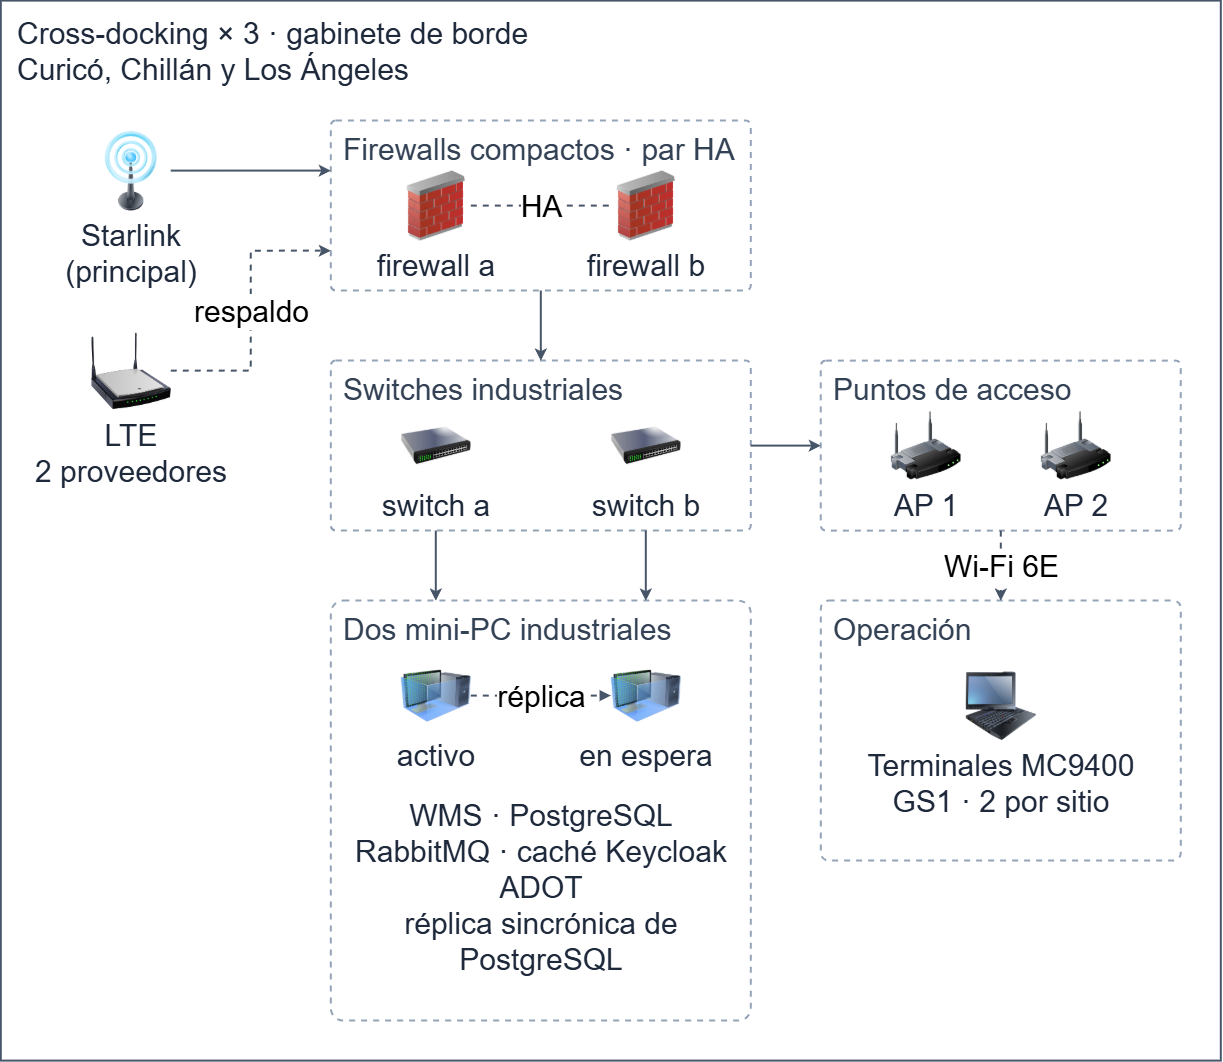
\includegraphics[width=\linewidth]{figuras/fisica/Arquitectura_Fisica_Crossdocking.png}
  \caption{Gabinete de borde de las plataformas de cross-docking}
  \label{fig:crossdocking}
  {\fontsize{9pt}{11pt}\selectfont\raggedright Fuente: elaboración a partir de Distribuidora Puelche S.A. (2026c, secciones~14.1--14.2 y~16.1, pp.~24--25 y~28--29), para volumetría y decisiones abiertas, y LafroX (2026d, diseño de este apartado, pp.~\pageref*{fuente-02-a-emplazamiento}--\pageref*{fuente-02-a-emplazamiento-fin}).\par}
\end{figure}
\FloatBarrier

Starlink es el enlace principal y el LTE de dos proveedores lo respalda. Ambos llegan a un par de firewalls compactos en alta disponibilidad, que termina el túnel VPN hacia la nube y conmuta de enlace en menos de 30 s. Detrás de los firewalls, dos switches industriales conectan los dos puntos de acceso de la nave y las dos interfaces de cada uno de los dos mini-PC industriales, que ejecutan en contenedores Docker el WMS, PostgreSQL, RabbitMQ, la caché de Keycloak y el colector ADOT. Los dos terminales inalámbricos de cada plataforma leen los códigos GS1 y trabajan contra el WMS local del mini-PC activo. El gabinete reúne en un par de equipos las funciones que Talca y Concepción reparten en varias máquinas virtuales, y con ello opera al 100\,\% en local la ventana de tres horas de recepción, desconsolidación y re-despacho. El mini-PC activo replica cada transacción en forma sincrónica al que está en espera, que toma su lugar si falla (RT-03.14, Bases Técnicas Transversales, cap. 3, p. 9; sección~\ref{sub:3-alta-disponibilidad}). Cada equipo tiene además alimentación redundante y dos SSD en RAID 1, y la reserva en Talca repone el equipo dañado. La reconstrucción desde el estado central de la nube, si fallan ambos, se trata en la sección~\ref{sec:conexiones}.

La Figura~\ref{fig:cd-concepcion} presenta el gabinete de borde del CD Concepción como parte de su operación autónoma.

\begin{figure}[htbp]
  \centering
  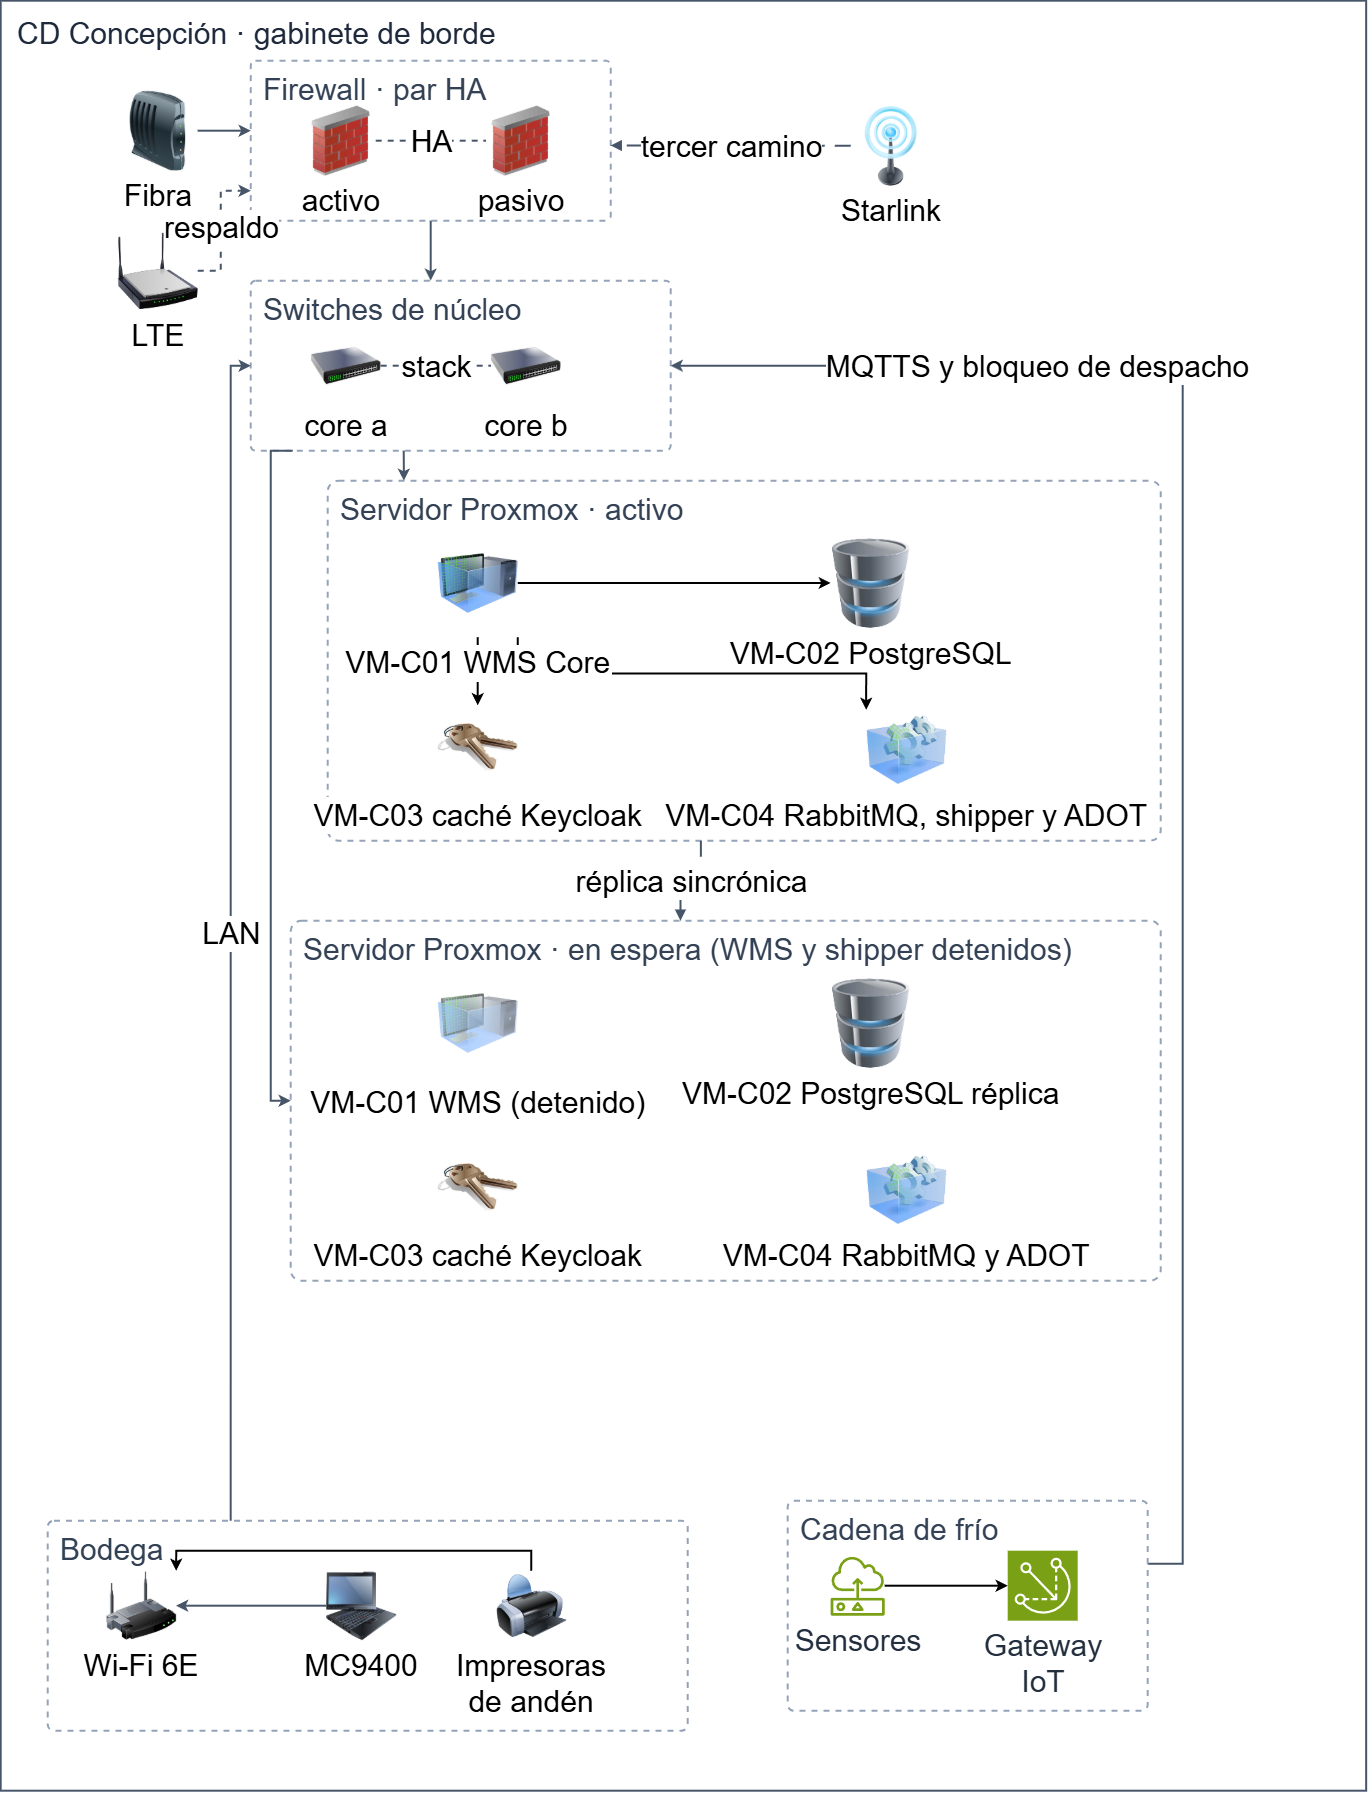
\includegraphics[width=\linewidth,height=0.88\textheight,keepaspectratio]{figuras/centros_de_datos/Arquitectura_Fisica_CD_Concepcion.png}
  \caption{Gabinete de borde del CD Concepción}
  \label{fig:cd-concepcion}
  {\fontsize{9pt}{11pt}\selectfont\raggedright Fuente: elaboración a partir de Distribuidora Puelche S.A. (2026c, secciones~14.1--14.2 y~16.1, pp.~24--25 y~28--29), para volumetría y decisiones abiertas, y LafroX (2026d, diseño de este apartado, pp.~\pageref*{fuente-02-a-emplazamiento}--\pageref*{fuente-02-a-emplazamiento-fin}).\par}
\end{figure}
\FloatBarrier

La figura sitúa el WMS, PostgreSQL, RabbitMQ y la caché de identidad en cuatro VM de un servidor Proxmox local. Un segundo servidor idéntico mantiene sus copias en espera, con la base replicada en forma sincrónica, y toma su lugar si falla (RT-03.14, Bases Técnicas Transversales, cap. 3, p. 9; sección~\ref{sub:3-alta-disponibilidad}). El par de firewalls y los dos switches de núcleo sostienen la red del sitio. Fibra D-03, LTE D-04 y Starlink D-06 proporcionan tres caminos hacia la nube. La UPS de 5 kVA del gabinete protege los dos servidores, los equipos de red y el terminal satelital durante 30 min y permite el apagado ordenado. Su carga de diseño, 3,42 kVA, usa el 68~\% de esa capacidad (Anexo 4-W). Cada servidor tiene fuentes redundantes. Solo si fallan ambos se repone el equipo y se reconstruye la base a partir del estado central alimentado por los eventos del propio sitio. El detalle de cada equipo está en el Formulario T-11.

La séptima instalación que proyecta el caso a tres años se incorpora parametrizando la infraestructura como código, sobre uno de los bloques de direccionamiento ya reservados en la Tabla~\ref{tab:t64}, sin obras en la sala de Talca.

En la nube, la región primaria es sa-east-1 y cada servicio se despliega en al menos dos zonas de disponibilidad. La región us-east-1 solo aloja la recuperación ante desastres. La Figura~\ref{fig:emplazamiento-dominios} ubica cada componente en su sitio.

\begin{figure}[htbp]
  \centering
  \LFXcuerpofigura\fontsize{9.2pt}{11.5pt}\selectfont
  \begin{tikzpicture}[
      caja/.style={draw=lafroxGris, line width=0.5pt, rounded corners=1.5pt,
                   inner sep=4pt, align=left, anchor=north west},
      titulo/.style={font=\intersemibold, anchor=north west, inner sep=0pt}]
    % Columna nube
    \node[titulo] at (0,0) {Nube AWS};
    \node[caja, text width=4.75cm] (sa) at (0,-0.5) {%
      \textbf{sa-east-1}, dos zonas o más\\[2pt]
      N-01 a N-03 Portales\\
      N-04 Plataforma de aplicación\\
      N-05 Base de datos en nube\\
      N-06 Telemetría cruda\\
      N-07 Caché\\
      N-08 Ingesta de IoT\\
      N-09 Mensajería\\
      N-10 Plataforma analítica\\
      N-11 Respaldo inmutable\\
      N-12 Seguridad y gobierno\\
      N-13 Gestión de dispositivos\\[3pt]
      Parte en nube de los híbridos};
    \node[caja, text width=4.75cm, below=5pt of sa.south west, anchor=north west] (us) {%
      \textbf{us-east-1}, recuperación\\[2pt]
      N-04 Réplica reducida\\
      N-05 Base secundaria\\
      N-06 Temperatura\\
      N-09 Colas preparadas\\
      N-10 Copia diferida\\
      N-11 Copia del respaldo\\
      N-12 Claves y secretos};
    % Columna on-premise
    \node[titulo] at (5.25,0) {On-premise};
    \node[caja, text width=5.3cm] (tal) at (5.25,-0.5) {%
      \textbf{CD Talca}, sala técnica secundaria\\[2pt]
      Máquinas VM-01 a VM-06\\
      con A-01 a A-05 y F-01\\
      Red: D-01 en par, D-02 a D-04 y D-06\\
      Respaldo: D-05\\
      Frío: B-01 y B-02\\
      Bodega: C-03 a C-05\\
      Gestión: F-02 y F-03};
    \node[caja, text width=5.3cm, below=5pt of tal.south west, anchor=north west] (con) {%
      \textbf{CD Concepción}, gabinete de borde\\[2pt]
      Dos servidores, activo y en espera:\\
      VM-C01 a VM-C04 y sus copias\\
      con A-01 a A-03, A-05 y F-01\\
      Red: D-01 a D-04 y D-06\\
      Frío: B-01 y B-02\\
      Bodega: C-03 a C-05\\
      Gestión: F-03};
    \node[caja, text width=5.3cm, below=5pt of con.south west, anchor=north west] (cdk) {%
      \textbf{Cross-docking}, tres sitios\\[2pt]
      Dos mini-PC E-01, activo y en espera\\
      con A-01 a A-03, caché de A-05 y F-01\\
      Red: D-01, D-02, D-04 y D-06\\
      Bodega: C-03\\
      Gestión: F-03};
    \node[caja, text width=5.3cm, below=5pt of cdk.south west, anchor=north west] (cm) {%
      \textbf{Casa matriz}, Talca\\[2pt]
      Sin cómputo. Usa la nube};
    % Columna terreno
    \node[titulo] at (11.05,0) {Terreno};
    \node[caja, text width=4.4cm] (calle) at (11.05,-0.5) {%
      \textbf{Calle}\\[2pt]
      C-01 App de preventa\\
      \quad 62 terminales EC55\\
      C-02 App de reparto\\
      \quad 96 terminales TC58e};
    \node[caja, text width=4.4cm, below=5pt of calle.south west, anchor=north west] (cam) {%
      \textbf{Camiones de frío}\\[2pt]
      B-03 Termógrafos, 28};
    \node[caja, text width=4.4cm, below=5pt of cam.south west, anchor=north west] (pts) {%
      \textbf{Locales de clientes}\\[2pt]
      14.200 puntos de entrega};
  \end{tikzpicture}
  \caption{Ubicación de los componentes por dominio y por sitio}
  \label{fig:emplazamiento-dominios}
  {\fontsize{9pt}{11pt}\selectfont\raggedright Fuente: elaboración a partir de Distribuidora Puelche S.A. (2026c, secciones~14.1--14.2 y~16.1, pp.~24--25 y~28--29), para volumetría y decisiones abiertas, y LafroX (2026d, diseño de este apartado, pp.~\pageref*{fuente-02-a-emplazamiento}--\pageref*{fuente-02-a-emplazamiento-fin}).\par}
\end{figure}

La figura muestra que cada instalación mantiene su operación local contra sus propios datos, dentro de las funciones y condiciones de 4.1.15 y del Anexo 4-J, aunque Concepción siga recibiendo parte de su surtido desde Talca. Esa autonomía no incluye emitir nuevas guías sin el ERP de Talca ni confirmar autorizaciones externas sin respuesta válida. Talca y Concepción tienen cada uno su WMS, su base, su broker y su caché de identidad. Los cross-docking reúnen esas mismas funciones en un par de mini-PC, uno activo y otro en espera. Y el terreno lleva su propio almacén local en el dispositivo. La nube concentra lo que es común a todos los sitios: los portales, el transaccional compartido, la analítica y los servicios de seguridad. Los doce componentes híbridos aparecen en los dos dominios porque cada uno tiene una parte que debe seguir operando en el sitio y otra que consolida en la nube.

\subsection{Correspondencia con la arquitectura lógica}

La \href{LAFROX-Subdocumento4-Anexos.pdf#tab:mapeo-logica}{Tabla A.14 del Anexo 4-N} asocia cada módulo y cada capa transversal de la arquitectura lógica del apartado 4.1 con el componente físico que lo ejecuta y con el lugar donde corre. Es la traza que permite seguir una responsabilidad lógica hasta su emplazamiento. Los componentes físicos se identifican con un catálogo único, agrupado por letra: A para el núcleo de bodega, B para la cadena de frío, C para los dispositivos de operación, D para la red, E para los cross-docking, F para la observabilidad y la seguridad de los nodos, y N para la nube.



El perfil local cubre M1, M2, M5, el bloqueo y la disposición sanitaria autorizada de M9 y la recepción física de retornos de M8 a través de la puerta de API local. Los módulos compartidos corren en N-04 y el terreno captura en su terminal. Los perfiles de ejecución se especifican en la sección \hyperref[sec:despliegue]{4.2.4}.

El recorrido de trazabilidad parte de la capacidad de 3.3–3.4, identifica su módulo y capa en 4.1 y llega al recurso de 4.2 y T-11. El \href{LAFROX-Subdocumento4-Anexos.pdf#anx:N}{Anexo 4-N} completa los doce módulos y los 37 componentes transversales con sus contratos y recursos, y el \href{LAFROX-Subdocumento4-Anexos.pdf#anx:E}{Anexo 4-E} enlaza las familias con las filas individuales de T-12. Un recurso que sirve a varios módulos conserva un identificador único. Compartir Fargate o PostgreSQL no fusiona sus responsabilidades.

\subsection{Síntesis del emplazamiento por dominio y criterio}

La Tabla~\ref{tab:t21} resume cómo se distribuyen los 36 componentes entre los tres dominios y los seis criterios del Artículo 16.2 (Bases Administrativas, art. 16.2, p. 11) que deciden cada emplazamiento. A continuación se justifica, dominio por dominio, por qué cada componente vive donde vive. El producto, la cantidad y la ubicación exacta de cada elemento no son materia del emplazamiento y se especifican en el Formulario T-11.

\Needspace{0.60\textheight}
\begin{tablalafrox}{Distribución de los componentes por dominio y criterio de emplazamiento}{tab:t21}%
  {Y H{0.15} H{0.15} H{0.15} H{0.15}}%
  {\cab{Criterio} & \cab{Nube pura} & \cab{On-premise} & \cab{Híbridos} & \cab{Total}}
  Latencia tolerada & 1 & 4 & 1 & 6 \\
  Criticidad operacional & 2 & 2 & 3 & 7 \\
  Volumen de datos & 3\textsuperscript{*} & --- & --- & 3 \\
  Conectividad & --- & 4 & 7 & 11 \\
  Regulación & 5 & --- & 1 & 6 \\
  Costo total de propiedad & 3\textsuperscript{*} & 1 & --- & 4 \\
  \textbf{Total de componentes} & \textbf{13} & \textbf{11} & \textbf{12} & \textbf{36} \\
\end{tablalafrox}

{\fontsize{9pt}{11pt}\selectfont\raggedright Fuente: elaboración a partir de Distribuidora Puelche S.A. (2026c, secciones~14.1--14.2 y~16.1, pp.~24--25 y~28--29), para volumetría y decisiones abiertas, y LafroX (2026d, diseño de este apartado, pp.~\pageref*{fuente-02-a-emplazamiento}--\pageref*{fuente-02-a-emplazamiento-fin}).\par}

El emplazamiento responde a cuatro criterios decisivos del caso:

\begin{itemize}
  \item Conectividad: decide once componentes y domina los on-premise e híbridos, por los cortes de enlace y el terreno sin señal.
  \item Regulación: decide seis y domina la nube pura, porque RT-03.22 no admite exponer servicios internos a Internet (Bases Técnicas Transversales, cap. 3, p. 10) y el Artículo 21.2 exige publicar solo por una capa de borde (Bases Administrativas, art. 21.2, p. 15).
  \item Costo y volumen: concentran en la nube lo que escala y se paga por uso.
  \item Latencia y criticidad: dejan en el sitio lo que debe responder sin enlace.
\end{itemize}

La columna Total suma 37 en las filas de criterios porque la plataforma analítica (N-10) se contabiliza en los dos criterios que deciden su emplazamiento, volumen de datos y costo total de propiedad. La fila final suma los 36 componentes efectivos.

\subsection{Componentes de nube pura}

Los trece componentes de nube pura viven solo en la nube. La justificación de cada uno y el criterio del Artículo 16.2 (Bases Administrativas, art. 16.2, p. 11) que la determina son los siguientes:

\begin{itemize}
  \item \textbf{N-01 Portal de Clientes} (regulación): atiendel catálogo, el pedido de autoatención, el estado de entrega, los documentos y el saldo de los clientes desde Internet, también como aplicación instalable que arma el pedido sin señal. Por eso se publica solo en la DMZ de la nube y ningún tráfico externo llega a los sitios del CLIENTE.
  \item \textbf{N-02 Portal de Transportistas} (regulación): desde la Etapa 2, los representantes de cada empresa transportista consultan rutas y documentos y confirman conductor y vehículo desde Internet, y ese acceso se resuelve en la DMZ de la nube. Los conductores externos no usan el portal: trabajan en la app de reparto con su identidad personal.
  \item \textbf{N-03 Portal de Proveedores} (regulación): los 180 proveedores consultan órdenes de compra, recepciones y devoluciones desde Internet, aislados de la red de bodega.
  \item \textbf{N-04 Plataforma de aplicación} (costo): Laravel corre en ECS Fargate con perfiles de API, reconciliación, trabajos y planificación que escalan por separado. La plataforma aloja el frontend Angular de consolas y el transporte AS2 de M11 en dos tareas distribuidas entre dos zonas cada uno. El motor de rutas M4 ejecuta una tarea por corrida, que ECS relanza en otra zona ante una falla para repetirla dentro de la planificación de 15:00 a 18:30, con el plazo de 20 min por corrida medido en la prueba de aceptación. M11 usa contratos versionados (ADR-11, Anexo 4-O).
  \item \textbf{N-05 Base de datos en nube} (criticidad): Aurora PostgreSQL guarda el transaccional de los módulos en nube y la réplica del WMS, conmuta entre zonas en menos de 30 s y se replica a us-east-1.
  \item \textbf{N-06 Telemetría cruda} (volumen): DynamoDB recibe las lecturas de temperatura sin gestión de capacidad y las expira a los 30 días, cuando ya están consolidadas en la capa analítica.
  \item \textbf{N-07 Caché} (latencia): ElastiCache mantiene en memoria el stock, el crédito y las sesiones para que la consulta de preventa responda en menos de 2 s.
  \item \textbf{N-08 Ingesta de IoT} (volumen): IoT Core recibe los 10.920 mensajes diarios de cadena de frío por MQTTS y gestiona los gateways del borde. Su motor de reglas escribe cada lectura en DynamoDB y publica en SNS las que superan el umbral.
  \item \textbf{N-09 Mensajería} (criticidad): una cola SQS FIFO recibe la reconciliación de los sitios como sobres JSON versionados, en orden por grupo y sin duplicados. Otra cola FIFO lleva las solicitudes al ERP hasta \texttt{erp-sync} y una cola FIFO de respuesta para Concepción y para cada cross-docking devuelve sus respuestas, porque Talca las recibe por RabbitMQ local. Una cola FIFO de coordinación por cada uno de los cinco sitios lleva las solicitudes de retención y liberación de stock que su shipper lee por conexión saliente. Otras colas SQS, separadas de esas, transportan los trabajos internos de Laravel, y SNS difunde las alertas de excursión térmica.
  \item \textbf{N-10 Plataforma analítica} (volumen y costo): S3, Glue, Redshift Serverless y QuickSight conservan 5 años de datos separados del transaccional. Los tableros y la autoría de QuickSight se integran en las consolas para usuarios registrados, con modelo semántico documentado, creación autónoma de informes, exportación y permisos separados de lectura y creación. Los indicadores operacionales actuales se consultan en la API de negocio.
  \item \textbf{N-11 Respaldo inmutable y réplica} (regulación): S3 Object Lock, AWS Backup y la réplica en us-east-1 guardan la copia que ni un administrador puede borrar y sostienen el RTO de 4 h y el RPO de 15 min.
  \item \textbf{N-12 Seguridad y gobierno} (regulación): KMS, Secrets Manager, WAF, Shield Advanced, Verified Access, Security Lake y CloudWatch implementan en la nube los controles del Artículo 21 de las Bases Administrativas (art. 21, p. 15) definidos en la arquitectura de seguridad (apartado 4.1), como servicios que un equipo de TI de cuatro personas puede operar.
  \item \textbf{N-13 Gestión de dispositivos} (costo): Android Enterprise y Zebra DNA gestionan como servicio el parque de terminales de preventa, reparto y cámara, con borrado remoto selectivo y sin infraestructura en los sitios.
\end{itemize}

Ningún componente de nube pura participa en las transacciones que el caso exige resolver sin enlace: la confirmación de preparación, el despacho y el registro de entrega se ejecutan en el sitio o en el dispositivo. Lo que sube a la nube lo hace por tres razones. Los portales y la gestión de identidades externas lo hacen por regulación, porque RT-03.22 no admite exponer servicios internos a Internet (Bases Técnicas Transversales, cap. 3, p. 10). La plataforma de aplicación, la analítica y la telemetría lo hacen por volumen y costo, porque su carga varía con la estación y se paga por uso. Y la seguridad y el respaldo lo hacen porque un equipo de TI de cuatro personas no puede operar esos controles en sus propios servidores.

\subsection{Componentes on-premise}

Los once componentes on-premise viven solo en las instalaciones del CLIENTE. La justificación de cada uno y su criterio:

\begin{itemize}
  \item \textbf{B-01 Sensores de temperatura} (latencia): los 21 puntos de medición de las cámaras se leen por Modbus en el mismo sitio, porque dentro de la cámara no hay señal y la lectura no puede esperar al enlace.
  \item \textbf{B-02 Gateway IoT} (latencia): los gateways de Talca y Concepción detectan la excursión crítica y sostenida y bloquean el despacho en menos de 5 s, con un buffer de 24 h si cae el enlace, igual a la autonomía del centro de distribución.
  \item \textbf{C-03 Terminales de bodega} (conectividad): los terminales MC9400 trabajan en la bodega y en las cámaras, incluido el congelado a $-$22\,\textdegree{}C, sin señal móvil, contra el WMS del sitio por la red inalámbrica de la bodega.
  \item \textbf{C-04 Impresoras de andén} (latencia): las seis impresoras ZT411 imprimen la etiqueta SSCC en el andén al armar la unidad logística, sin salir de la red local.
  \item \textbf{C-05 Balanzas de recepción} (latencia): las tres balanzas envían el peso de recepción al WMS del sitio en línea, sin digitación y sin depender del enlace.
  \item \textbf{D-02 Switching} (criticidad): los switches de cada sitio segmentan la red local por VLAN y la mantienen operativa aunque caiga la WAN.
  \item \textbf{D-03 Enlace de fibra} (conectividad): es el camino principal de la VPN en Talca y Concepción, con 20 y 10 Mbps en régimen.
  \item \textbf{D-04 Enlace LTE} (conectividad): respalda la fibra en los CD y, con dos proveedores, respalda a Starlink en los cross-docking, con conmutación en menos de 30 s.
  \item \textbf{D-06 Enlace satelital} (conectividad): Starlink es el camino principal de los cross-docking, respaldado por LTE de dos proveedores, y el tercer camino en espera caliente de Talca y Concepción, con terminal encendido, túnel IPsec establecido y BGP de menor preferencia que solo toma tráfico si fallan fibra y LTE.
  \item \textbf{E-01 WMS de cross-docking} (criticidad): el par de mini-PC de cada plataforma, uno activo y otro en espera, opera 100\,\% en local la ventana de 3 h de recepción, desconsolidación y re-despacho, con su propio broker y su propia base, replicada al equipo en espera.
  \item \textbf{F-02 Gestión de parches} (costo): Ansible aplica los parches y las líneas base CIS a los nodos de los cinco sitios por la red de gestión, sin licencia de plataforma.
\end{itemize}

En el on-premise dominan la latencia y la conectividad. Los sensores, las impresoras, las balanzas y los terminales de cámara son periféricos que trabajan donde está la mercadería, y ninguno puede depender de un enlace que el caso describe como intermitente. Los tres enlaces y el switching tampoco podrían emplazarse en otro lugar: son la infraestructura que conecta el sitio con la nube y sostiene su red interna cuando esa conexión falla.

LafroX acuerda con la Contraparte Técnica del CLIENTE la ventana de cada aplicación de parches y líneas base CIS en los sitios, dentro de la programación de mantenimiento y respetando los congelamientos y las ventanas protegidas de 4.2.4.1.4. Ansible aplica el cambio con respaldo, verificación y reversión preparados, y el resultado queda registrado en la gestión de configuración (RT-03.15, Bases Técnicas Transversales, cap. 3, p. 9).

\subsection{Componentes híbridos}

Los doce componentes híbridos tienen una parte en cada dominio. Para cada uno, la justificación explica qué parte vive en el sitio, qué parte vive en la nube y por qué se reparten así:

\begin{itemize}
  \item \textbf{A-01 Motor WMS} (latencia): el perfil \texttt{wms\_only} del artefacto Laravel, con su servidor web y PHP-FPM, corre en VM-01, VM-C01 y E-01 porque la confirmación de preparación debe responder en 1 s sin depender del enlace, y su réplica en Aurora sostiene la continuidad. El mismo motor expone la puerta de API local de la bodega, que durante un corte valida el esquema, la tasa, el UUID y la auditoría de las solicitudes de los terminales sin pasar por API Gateway.
  \item \textbf{A-02 Base transaccional del WMS} (criticidad): PostgreSQL 16 en VM-02 y VM-C02 es el registro de cada bodega durante un corte. AWS DMS replica continuamente los cambios de VM-02 (Talca) a Aurora para continuidad y lectura por fibra, LTE o Starlink. VM-C02 (Concepción) entrega sus eventos por las colas de integración. En Concepción y en cada cross-docking, la base activa se replica en forma sincrónica al equipo en espera.
  \item \textbf{A-03 Broker de colas} (conectividad): RabbitMQ en VM-03, VM-C04 y E-01 guarda hasta 24 h de eventos sin enlace, con mensajes persistentes y confirmación de publicación. El shipper, un proceso PHP con el adaptador AMQP \texttt{php-amqplib}, los publica como sobres JSON en SQS FIFO y solo los retira del broker cuando SQS confirma la recepción. El outbox conserva 24 h de eventos ya enviados para reenviarlos tras una conmutación.
  \item \textbf{A-04 Capa anticorrupción del ERP} (criticidad): corre en VM-04, en la misma sala que el ERP de 2017, que no se modifica. En la misma VM, \texttt{erp-sync} consume la cola local de Talca y, mediante conexión saliente, la cola FIFO de solicitudes al ERP de los demás orígenes, cuyas respuestas devuelve por la cola de cada sitio. Usa una clave idempotente por operación para que un reintento no emita un segundo documento tributario.
  \item \textbf{A-05 Identidad} (conectividad): el IdP maestro Keycloak corre en Fargate y sus cachés de solo lectura en VM-05, VM-C03 y E-01 validan las sesiones de bodega y de cross-docking sin enlace. En el mismo nodo, un verificador local habilita cada relevo de turno durante un corte con el manifiesto de turno firmado y un segundo factor local, el PIN personal.
  \item \textbf{B-03 Termógrafos de camión} (conectividad): los 28 termógrafos —18 en los camiones propios y 10 en los de los transportistas, instalados con el acuerdo de cada uno (S-28)— registran la temperatura durante toda la ruta sin señal y la difunden por Bluetooth. El terminal del conductor la lee, evalúa la regla de excursión, alerta en la cabina en el momento y reenvía la alerta a la nube por la red celular, de inmediato con cobertura o al recuperarla. Al volver el camión, el mismo terminal descarga el registro completo, comprueba su control de integridad y lo envía a la nube para que IoT Core lo valide.
  \item \textbf{C-01 App de preventa} (conectividad): toma pedidos contra el almacén local del terminal cuando no hay señal y sincroniza por CloudFront al reconectar, sin duplicar pedidos (sección~\ref{sec:conexiones}).
  \item \textbf{C-02 App de reparto} (conectividad): registra entregas, evidencia y cobros durante 14 h sin señal y los sincroniza con la nube al recuperar cobertura.
  \item \textbf{D-01 Firewall y Customer Gateway} (criticidad): el par de firewalls de cada uno de los cinco sitios termina los túneles IPsec hacia el Transit Gateway de AWS y conmutan de enlace en menos de 30 s.
  \item \textbf{D-05 Respaldo local} (conectividad): el NAS WORM de Talca restaura el WMS en 4 h sin depender del enlace, y su complemento inmutable vive en S3 Object Lock.
  \item \textbf{F-01 Telemetría de observabilidad} (conectividad): los colectores ADOT de VM-06, VM-C04 y E-01 guardan hasta 24 h de métricas y trazas en disco y las envían a CloudWatch al reconectar.
  \item \textbf{F-03 Detección en endpoints} (regulación): los agentes EDR de cada nodo y estación reportan a una consola central, lo que da una sola respuesta ante incidentes en nube y on-premise. El servidor del ERP es un activo del CLIENTE que no forma parte de la solución: LafroX lo traslada sin cambiar su software, y el firewall de Talca restringe las entradas al tráfico de la ACL en VM-04 y a la administración autorizada del CLIENTE. Permite las salidas tributarias del ERP hacia el SII por los caminos habilitados, con destinos, puertos y reglas documentados en el levantamiento de INT-07. Esto no habilita escrituras directas de los módulos al ERP.
\end{itemize}

Los componentes híbridos siguen todos el mismo patrón: la parte que atiende la operación queda en el sitio y la parte que consolida queda en la nube, unidas por un mecanismo que tolera el corte. En el núcleo de bodega, Talca replica su base por DMS y los demás sitios sincronizan eventos por colas. En el terreno, el almacén local del dispositivo. Y en la observabilidad, el buffer en disco de los colectores. Por eso la conectividad es el criterio dominante en siete de los doce: cada uno existe en dos lugares precisamente porque el enlace entre ellos no es confiable.

\subsection{Autonomía de cada ámbito sin enlace}

El emplazamiento descrito se verifica en lo que cada ámbito puede hacer cuando pierde el enlace. El listado \hyperref[tab:t29]{de autonomía por ámbito} declara esa autonomía y el tiempo en que cada ámbito vuelve a quedar sincronizado.

\paragraph*{Autonomía por ámbito ante la pérdida del enlace}
\phantomsection
\label{tab:t29}
\begin{itemize}
\item \textbf{Centros de distribución de Talca y Concepción.} \textbf{Autonomía sin enlace:} 24 h o más, con reconciliación determinista.
\item \textbf{Terreno.} \textbf{Autonomía sin enlace:} 14 h, un turno completo.
\item \textbf{Cross-docking.} \textbf{Autonomía sin enlace:} 24 h o más. La ventana de 3 h opera 100\,\% local.
\item \textbf{Sincronización al reconectar.} \textbf{Autonomía sin enlace:} CD en 2 h, flota en 10 min.
\end{itemize}

{\fontsize{9pt}{11pt}\selectfont\raggedright Fuente: elaboración a partir de Distribuidora Puelche S.A. (2026c, secciones~14.1--14.2 y~16.1, pp.~24--25 y~28--29), para volumetría y decisiones abiertas, y LafroX (2026d, diseño de este apartado, pp.~\pageref*{fuente-02-a-emplazamiento}--\pageref*{fuente-02-a-emplazamiento-fin}).\par}

Durante la autonomía, cada ámbito mantiene las funciones habilitadas contra sus datos locales, con permisos vigentes, bloqueos sanitarios y las condiciones del Anexo 4-J:

\begin{itemize}
\item El centro de distribución sigue con recepción, preparación, conteo cíclico y trazabilidad contra la base local. El despacho exige una guía válida que ampare la carga y una autorización sanitaria vigente. Calidad dispone los lotes del sitio desde su perfil Kotlin autorizado y con evidencia local suficiente. Si falta permiso o evidencia, el bloqueo continúa. Una nueva guía requiere ERP y comunicación tributaria. La falta de conexión no equivale a autorización.
  \item El terreno sigue con toma de pedido, entrega, evidencia, devoluciones y cobros contra el almacén local del dispositivo.
  \item El cross-docking mantiene recepción, desconsolidación, lectura del termógrafo en la recepción y re-despacho.
\end{itemize}

Al reconectar, el vuelco ocurre en orden estricto, sin duplicados y con reconciliación determinista.

Las seis horas del peor corte de fibra de Talca quedan dentro de las 24 horas del centro de distribución. En terreno se distinguen las 14 horas de captura autorizada sin señal de la ventana física de ruta de hasta 14,5 horas de 4.2.1.2. El inicio y término de la credencial se registran por turno: una ruta que exceda su vigencia requiere renovación con conexión. La batería y el registro continuo del termógrafo no amplían los permisos. Los tiempos de sincronización se sostienen con los enlaces dimensionados en la sección~\ref{sec:dimensionamiento}, y lo que ocurre ante cada falla se desarrolla en la sección~\ref{sec:conexiones}.

\label{fuente-02-a-emplazamiento-fin}
